\documentclass[tikz,border=10pt]{standalone}
\usetikzlibrary{calc}
\usepackage{tikz-dimline} % Import tikz-dimline package
\begin{document}

%Similar Cones
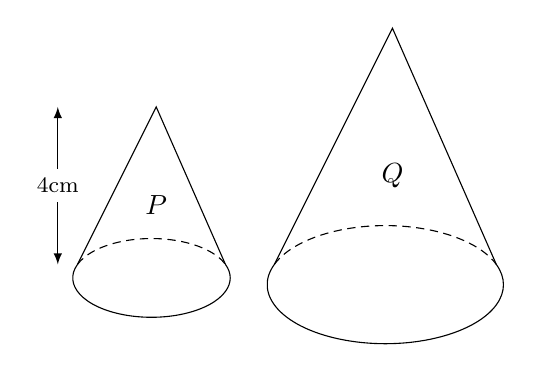
\begin{tikzpicture}
%Draw first cone
    \def\scaleFactor{1.5}
    \draw (-1,0) arc (160:380:1cm and 0.5cm) -- (0,2) -- cycle;
    \draw[densely dashed] (-1,0) arc (160:20:1cm and 0.5cm);
    %Label cone 1
    \node (P) at (0,0.75) {$P$};

Draw the second cone, scaled by 1.5
  \begin{scope}[shift={(3cm,0)}, scale=\scaleFactor]
    \draw (-1,0) arc (160:380:1cm and 0.5cm) -- (0,2) -- cycle;
    \draw[densely dashed] (-1,0) arc (160:20:1cm and 0.5cm);
    %Label cone 2
    \node (Q) at (0,0.75) {$Q$};
  \end{scope}

    
   % Dimensions using tikz-dimline
    
    % Height dimension for cone P
    \dimline[label style={sloped=false}, line style={<->,>=latex, scale =2}, extension start length=0, extension end length=0]{(-1.25,0)}{(-1.25,2)}{\footnotesize 4cm}

\end{tikzpicture}

%Frustrum of cones
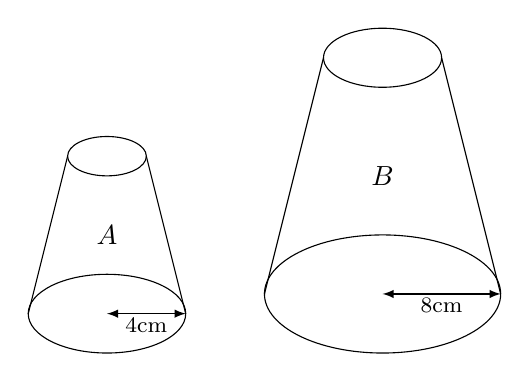
\begin{tikzpicture}[scale = 1]
    % Define the scale factor
    \def\scaleFactor{1.5}

    % Draw the first frustum
    \draw (1,1) ellipse [x radius=1cm,y radius=.5cm];
    \draw (1,3) ellipse [x radius=0.5cm,y radius=.25cm];
    \draw (0,1) -- (0.5,3);
    \draw (2,1) -- (1.5,3);
    % Label frustum A
    \node at (1,2) {$A$};

    % Dimensions using tikz-dimline for frustum A
    \dimline[label style={sloped=false, fill=none, yshift = -0.15cm}, line style={<->,>=latex}, extension start length=0, extension end length=0] 
    {(1,1)}{(2,1)}{\footnotesize 4cm};

    
    % Draw the second frustum, scaled by 1.5
    \begin{scope}[shift={(3cm,-0.25)}, scale=\scaleFactor]
         \draw (1,1) ellipse [x radius=1cm,y radius=.5cm];
        \draw (1,3) ellipse [x radius=0.5cm,y radius=.25cm];
        \draw (0,1) -- (0.5,3);
        \draw (2,1) -- (1.5,3);
        % Label frustum B
        \node at (1,2) {$B$};

        % Dimensions using tikz-dimline for frustum B
        \dimline[label style={sloped=false, fill=none, yshift = -0.15cm}, line style={<->,>=latex}, extension start length=0, extension end length=0] 
    {(1,1)}{(2,1)}{\footnotesize 8cm};
    \end{scope}
    
\end{tikzpicture}

%Similar Cylinders
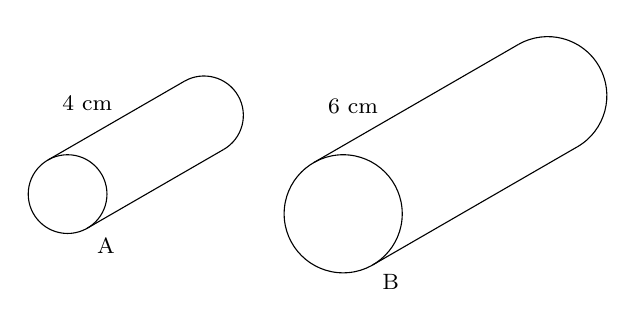
\begin{tikzpicture}[scale = 1]
    % Define dimensions
    \def\cylinderHeight{2cm}  % Height of the cylinder
    \def\circleRadius{0.5} % radius of small circle (front face)
    \def\scaleFactor{1.5}

    %Drawing small cylinder
    \draw (0,0) circle [radius = \circleRadius];
    \path (0,0) ++(120:\circleRadius) coordinate (A);
    \path (0,0) ++(-60:\circleRadius) coordinate (B);
    \path (0,0) -- ++(30:\cylinderHeight) coordinate (L);
    \draw (A) -- ++(30:\cylinderHeight);
    \draw (B) -- ++(30:\cylinderHeight) coordinate (K);
    \draw (K) arc [start angle=-60,   end angle=120, radius = 0.5cm];

    %Labels
    \node at (B) [anchor = north west] {\footnotesize A};
    \node at (A) [anchor = south, yshift= 0.5cm, xshift = 0.5cm] {\footnotesize 4 cm};

     % Draw the second cylinder, scaled by 1.5
    \begin{scope}[shift={(3.5cm,-0.25)}, scale=\scaleFactor]
         \draw (0,0) circle [radius = \circleRadius];
        \path (0,0) ++(120:\circleRadius) coordinate (A);
        \path (0,0) ++(-60:\circleRadius) coordinate (B);
        \path (0,0) -- ++(30:\cylinderHeight) coordinate (L);
        \draw (A) -- ++(30:\cylinderHeight);
        \draw (B) -- ++(30:\cylinderHeight) coordinate (K);
        \draw (K) arc [start angle=-60,   end angle=120, radius = 0.5cm];

        %Labels
        \node at (B) [anchor = north west] {\footnotesize B};
        \node at (A) [anchor = south, yshift= 0.5cm, xshift = 0.5cm] {\footnotesize 6 cm};
    \end{scope}

\end{tikzpicture}

%Frustrums of cones II
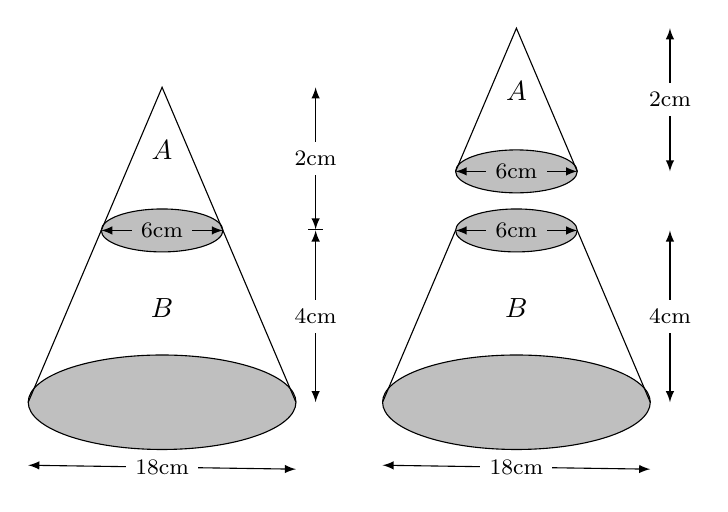
\begin{tikzpicture}[scale = 1]
    % Define the parameters
    \def\scaleFactor{1}
    \def\yRadiusA{0.6}
    \def\xRadiusA{1.7}
    \def\coneHeight{4}
    \def\ratio{2.2} %ratio : 1 FullconeHeight : small cone
    \def\yRadiusB{\yRadiusA / \ratio}
    \def\xRadiusB{\xRadiusA / \ratio}
    \def\frustrumHeight{\coneHeight - \coneHeight * 1/ \ratio}
    
    
    % Draw the first frustum
    \draw[fill = gray!50] (1,1) ellipse [x radius=\xRadiusA,y radius=\yRadiusA];
    \draw[fill = gray!50] (1,1 + \frustrumHeight) ellipse [x radius=\xRadiusB,y radius=\yRadiusB];

    %Draw edges
    \draw (1-\xRadiusA,1) -- (1-\xRadiusB,1+\frustrumHeight);
    \draw (1+\xRadiusA,1) -- (1+\xRadiusB,1+\frustrumHeight);
    %Small Cone
    \draw (1-\xRadiusB, 1+\frustrumHeight) -- (1,\coneHeight + 1) -- (1+\xRadiusB, 1+\frustrumHeight);
    %label small cone
    \node at (1,0.8*\coneHeight + 1) {$A$};
    % Label frustum
    \node at (1,0.3*\coneHeight + 1) {$B$};

    % Dimensions using tikz-dimline for frustum 1
    \dimline[label style={sloped=false}, line style={<->,>=latex}, extension start length=0, extension end length=0] 
    {(1-\xRadiusA,1 - \yRadiusA - 0.2)}{(1 + \xRadiusA,1 - \yRadiusA - 0.25)}{\footnotesize 18cm};
    \dimline[label style={sloped=false, fill = gray!50}, line style={<->,>=latex}, extension start length=0, extension end length=0] 
    {(1-\xRadiusB,1 + \frustrumHeight)}{(1 + \xRadiusB,1 + \frustrumHeight)}{\footnotesize 6cm};
    \dimline[label style={sloped=false}, line style={<->,>=latex}, extension start length=0, extension end length=0] 
    {(1 + \xRadiusA + 0.25, 1)}{(1 + \xRadiusA + 0.25, 1 + \frustrumHeight)}{\footnotesize 4cm};
    \dimline[label style={sloped=false}, line style={|<->,>=latex}, extension start length=0, extension end length=0] 
    {(1 + \xRadiusA + 0.25, 1 + \frustrumHeight)}{(1 + \xRadiusA + 0.25, 1 + \coneHeight)}{\footnotesize 2cm};

    
    % Draw the copy of frustum 1
    \begin{scope}[shift={(4.5cm,0)}, scale=\scaleFactor]
         \draw[fill = gray!50] (1,1) ellipse [x radius=\xRadiusA,y radius=\yRadiusA];
        \draw[fill = gray!50] (1,1 + \frustrumHeight) ellipse [x radius=\xRadiusB,y radius=\yRadiusB];
    
        %Draw edges
        \draw (1-\xRadiusA,1) -- (1-\xRadiusB,1+\frustrumHeight);
        \draw (1+\xRadiusA,1) -- (1+\xRadiusB,1+\frustrumHeight);
        % Label Frustrum
        \node at (1,0.3*\coneHeight + 1) {$B$};
        
    
        % Dimensions using tikz-dimline for frustum 1
        \dimline[label style={sloped=false}, line style={<->,>=latex}, extension start length=0, extension end length=0] 
        {(1-\xRadiusA,1 - \yRadiusA - 0.2)}{(1 + \xRadiusA,1 - \yRadiusA - 0.25)}{\footnotesize 18cm};

        \dimline[label style={sloped=false, fill = gray!50}, line style={<->,>=latex}, extension start length=0, extension end length=0] 
    {(1-\xRadiusB,1 + \frustrumHeight)}{(1 + \xRadiusB,1 + \frustrumHeight)}{\footnotesize 6cm};
      \dimline[label style={sloped=false}, line style={<->,>=latex}, extension start length=0, extension end length=0] 
    {(1 + \xRadiusA + 0.25, 1)}{(1 + \xRadiusA + 0.25, 1 + \frustrumHeight)}{\footnotesize 4cm};
    \end{scope}

    \begin{scope}[shift={(4.5,0.75)}, scale=\scaleFactor]
         %Small Cone
         \draw[fill = gray!50] (1,1 + \frustrumHeight) ellipse [x radius=\xRadiusB,y radius=\yRadiusB];
        \draw (1-\xRadiusB, 1+\frustrumHeight) -- (1,\coneHeight + 1) -- (1+\xRadiusB, 1+\frustrumHeight);

        %label small cone
        \node at (1,0.8*\coneHeight + 1) {$A$};

        %Mark dimensions
        \dimline[label style={sloped=false, fill = gray!50}, line style={<->,>=latex}, extension start length=0, extension end length=0] 
        {(1-\xRadiusB,1 + \frustrumHeight)}{(1 + \xRadiusB,1 + \frustrumHeight)}{\footnotesize 6cm};

        \dimline[label style={sloped=false}, line style={<->,>=latex}, extension start length=0, extension end length=0] 
    {(1 + \xRadiusA + 0.25, 1 + \frustrumHeight)}{(1 + \xRadiusA + 0.25, 1 + \coneHeight)}{\footnotesize 2cm};
    \end{scope}

\end{tikzpicture}

%Semi cylinder on cuboid
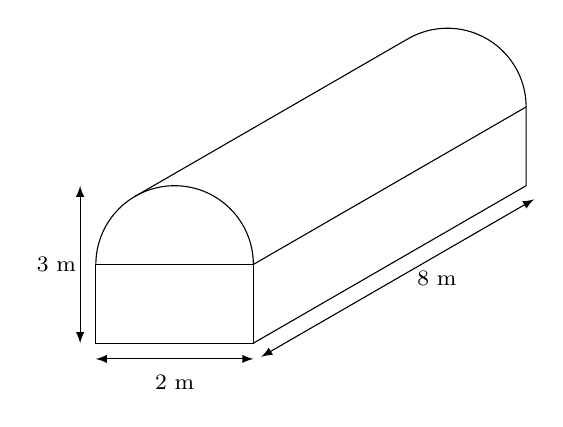
\begin{tikzpicture}[scale = 1]
    % Define dimensions
    \def\cylinderHeight{4cm}  % Height of the cylinder
    \def\cylinderRadius{1} % radius of small circle (front face)
    \def\cuboidHeight{1}
    \def\scaleFactor{3}
    \def\angle{30} %angle of perspective of object

    %Drawing semi cylinder
    \draw (0,0) arc [start angle=0,   end angle=180, radius = \cylinderRadius] coordinate (C);
    \path (0,0) arc [start angle=0,   end angle=120, radius = \cylinderRadius] coordinate (K);
    \draw (K) -- ++(\angle:\cylinderHeight) coordinate (B);
    \draw (0,0) -- ++(\angle:\cylinderHeight) coordinate (L);
    \draw (L) arc [start angle=0,   end angle=120, radius = \cylinderRadius];

    %Drawing cuboid
    \draw (0,0) -- (C) -- ++(-90:\cuboidHeight) -- ++(0:2* \cylinderRadius) coordinate (L) -- cycle;
    \draw (L) -- ++(\angle:\cylinderHeight) coordinate (P) -- ++(90:\cuboidHeight);
    %Dimension
    \dimline[label style={sloped=false, fill = none, xshift= -0.3cm}, line style={<->,>=latex}, extension start length=0, extension end length=0] 
    {(-2* \cylinderRadius - 0.2, -\cuboidHeight)}{(-2* \cylinderRadius - 0.2, \cylinderRadius)}{\footnotesize 3 m};

    \dimline[label style={sloped=false, fill = none, yshift= -0.3cm}, line style={<->,>=latex}, extension start length=0, extension end length=0] 
    {(0, -\cuboidHeight - 0.2)}{(-2* \cylinderRadius , -\cuboidHeight - 0.2)}{\footnotesize 2 m};

    \dimline[label style={sloped=false, fill = none, xshift = 0.5cm}, line style={<->,>=latex}, extension start length=0, extension end length=0] 
    {($(L)!.2cm!-90:(P)$)}{($(P)!.2cm!90:(L)$)}{\footnotesize 8 m};
    
\end{tikzpicture}

%Semi cylinder
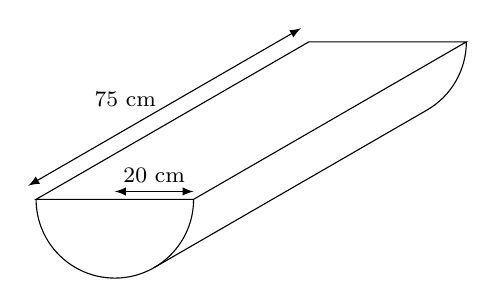
\begin{tikzpicture}[scale = 1]
    % Define dimensions
    \def\cylinderHeight{4cm}  % Height of the cylinder
    \def\cylinderRadius{1} % radius of small circle (front face)
    \def\cuboidHeight{1}
    \def\scaleFactor{3}
    \def\angle{30} %angle of perspective of object

    %Drawing semi cylinder
    \draw (0,0) arc [start angle=360,   end angle=180, radius = \cylinderRadius] coordinate (C);
    \path (0,0) arc [start angle=360,   end angle=300, radius = \cylinderRadius] coordinate (K);
    \draw (K) -- ++(\angle:\cylinderHeight) coordinate (B);
    \draw (0,0) -- ++(\angle:\cylinderHeight) coordinate (L) -- ++(180 : 2*\cylinderRadius) coordinate (Q) -- (C) -- (0,0);
    \draw (L) arc [start angle=360,   end angle=300, radius = \cylinderRadius];

    \dimline[label style={sloped=false, fill = none, yshift= 0.2cm}, line style={<->,>=latex}, extension start length=0, extension end length=0] 
    {(0, 0.1)}{(-\cylinderRadius , 0.1)}{\footnotesize 20 cm};

    \dimline[label style={sloped=false, fill = none, xshift = -0.5cm, yshift = 0.1cm}, line style={<->,>=latex}, extension start length=0, extension end length=0] 
    {($(C)!-.2cm!-90:(Q)$)}{($(Q)!-.2cm!90:(C)$)}{\footnotesize 75 cm};
    
\end{tikzpicture}
%cube stacks
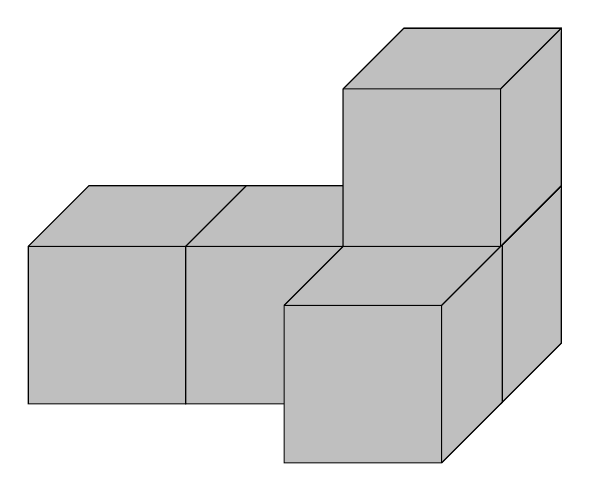
\begin{tikzpicture}[scale = 1]
\newcommand{\cube}[3][fill=white]{
    \draw[black, #1] (#2) -- ++(-#3,0,0) -- ++(0,#3,0) -- ++(0,0,-#3) -- ++(#3,0,0) -- ++(0,-#3,0)-- cycle;
    \draw[black,line join=bevel, #1] (#2) -- ++(0,#3,0) -- ++(0,0,-#3) (#2)++(0,#3,0)--++(-#3,0,0);
}

\cube[fill=gray!50]{0,0,0}{2}

\begin{scope}[xshift=2cm]
    \cube[fill=gray!50]{0,0,0}{2}
\end{scope}
\begin{scope}[xshift=4cm]
    \cube[fill=gray!50]{0,0,0}{2}
\end{scope}
\begin{scope}[xshift=4cm, yshift = 2cm]
    \cube[fill=gray!50]{0,0,0}{2}
\end{scope}
\begin{scope}[xshift=3.25cm, yshift = -0.75cm]
    \cube[fill=gray!50]{0,0,0}{2}
\end{scope}
\begin{scope}[xshift=4cm, yshift = 2cm]
    \cube[fill=gray!50]{0,0,0}{2}
\end{scope}
\end{tikzpicture}

%cuboid boxes with labels
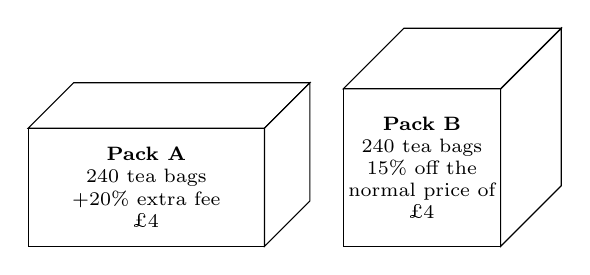
\begin{tikzpicture}[scale=1]
    \pgfmathsetmacro{\cubex}{3}
    \pgfmathsetmacro{\cubey}{1.5}
    \pgfmathsetmacro{\cubez}{1.5}
\draw (0,0,0) -- ++(-\cubex,0,0) -- ++(0,-\cubey,0) -- ++(\cubex,0,0) -- cycle;
\draw (0,0,0) -- ++(0,0,-\cubez) -- ++(0,-\cubey,0) -- ++(0,0,\cubez) -- cycle;
\draw (0,0,0) -- ++(-\cubex,0,0) -- ++(0,0,-\cubez) -- ++(\cubex,0,0) -- cycle;

     % Label for the first cuboid
    \node[align=center, font=\scriptsize] at (-\cubex/2, -\cubey/2, 0) {\textbf{Pack A}\\ 240 tea bags\\ $+$20\% extra fee \\ \pounds$4$};
    
    \begin{scope}[xshift = 3cm, yshift = 0.5cm]
    \pgfmathsetmacro{\cubex}{2}
    \pgfmathsetmacro{\cubey}{2}
    \pgfmathsetmacro{\cubez}{2}
    \draw (0,0,0) -- ++(-\cubex,0,0) -- ++(0,-\cubey,0) -- ++(\cubex,0,0) -- cycle;
    \draw (0,0,0) -- ++(0,0,-\cubez) -- ++(0,-\cubey,0) -- ++(0,0,\cubez) -- cycle;
    \draw (0,0,0) -- ++(-\cubex,0,0) -- ++(0,0,-\cubez) -- ++(\cubex,0,0) -- cycle;

    \node[align=center, font=\scriptsize] at (-\cubex/2, -\cubey/2, 0) {\textbf{Pack B}\\ 240 tea bags\\ 15\% off the \\ normal price of \\ \pounds$4$};
    \end{scope}

\end{tikzpicture}

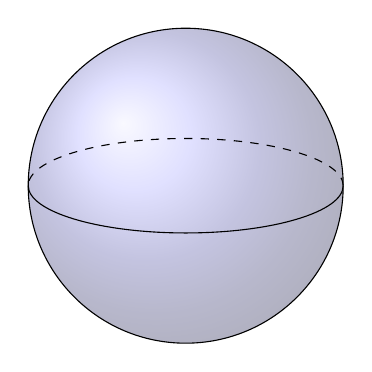
\begin{tikzpicture}
  \shade[ball color = blue!40, opacity = 0.4] (0,0) circle (2cm);
  \draw (0,0) circle (2cm);
  \draw (-2,0) arc (180:360:2 and 0.6);
  \draw[dashed] (2,0) arc (0:180:2 and 0.6);

\end{tikzpicture}

\end{document}


